\section{Experimental Evaluation}
\label{sec:simulation}

The experiment studies the effect of an increasing penetration rate
of vehicular automation technology.  Suppose human-driven vehicles are
gradually replaced by a particular type of semi-autonomous vehicle or
fully autonomous vehicle until all vehicles become that type.  We examine how
much benefit SemiAIM provides during the transition period.

In this experiment, the traffic consisted of one of the three types of
vehicles we defined in Section~\ref{sec:vehicles} as well as fully
autonomous (Type A) and human-driven (Type H) vehicles.  We measured
the traffic delay as we gradually increased the ratio of
\mbox{(semi-)autonomous} vehicles to human-driven vehicles while
keeping the traffic level at 360 vehicles/hour/lane.  We repeated the
simulation 30 times for 1800s during each time.  For each run, we
measured the average delay of all vehicles.  The average delays are
shown in Figure~\ref{fig:two360}.  Each data point in the figure is an
average of 30 values, and the error bar is the 95\% confident interval.

 
\begin{figure}
\centering
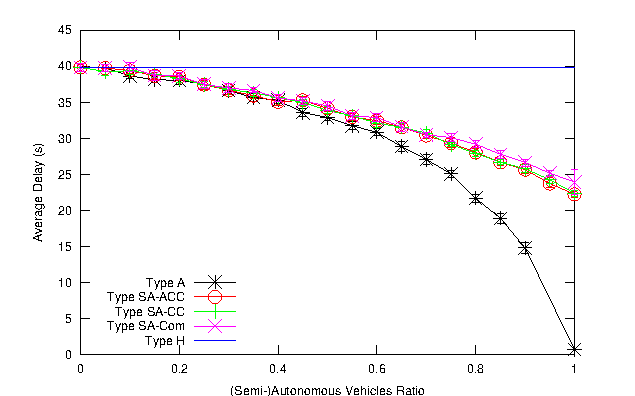
\includegraphics[width=0.9\columnwidth]{figures/figure_1.pdf}
\vspace{-.07in}
\caption{(Semi-)Autonomous vehicles vs. Human-Driven vehicles. Traffic
level = 360 vehicles/lane/hour.}
\label{fig:two360}
\vspace{-.1in}
\end{figure}

According to Figure~\ref{fig:two360}, the performance of
semi-autonomous vehicles is very similar to fully autonomous vehicles
when the ratio to human-driven vehicles is below 40\%.  However, when
the ratio increases beyond 40\%, fully autonomous vehicles
increasingly outperform semi-autonomous vehicles.  Previous studies
showed that FCFS-Signal needs at least 90\% of fully autonomous
vehicles in the traffic in order to be fully
effective~\cite{mybib:Dresner07Sharing}.  We successfully replicate the
result, observing that the average delay drops rapidly when the
traffic has more than 90\% fully autonomous vehicles, and approaches
zero when all vehicles are fully autonomous.  Semi-autonomous vehicles
cannot achieve the same dramatic decrease in traffic delay, but they,
with the help of SemiAIM, manage to reduce the delay by 46\% (from
39.9s to 22.4s) compared to human-driven vehicles.  As expected, in
the presence of semi-autonomous vehicles, SemiAIM provides significant
advantages even when there are no fully autonomous vehicles on the
road.
Another observation is that both Type SA-ACC and Type SA-CC vehicles
have a significantly lower average delay than Type SA-Com vehicles.

